% //TODO:真空ポンプを用いた場合と電磁石を用いた把持方法の比較文章を書く
\section{実験装置の改良による影響に関して}
\label{sec:reexp}

先行研究\cite{ref:8}において,電磁石を用いて,磁力によって球の把持を行っていた.一方で,本研究において,強磁性体以外の球の把持を行うため,真空ポンプを用いて吸引する手法に変更した.その把持手法の変化に伴う影響を議論する.

% Fig.\ref{fig:re-exp-vaccume}に真空ポンプを用いた把持方法における再現性の確認の実験結果を示す.縦軸は落下速度,横軸は落下開始時からの経過時間である.この再現性確認において,溶液の再作成から行った.終端速度に達するまでの経過はほぼ同様であった.一方で,終端速度は約10\%の誤差が生じた.これは,溶液の作製による誤差の影響を受けていると考えられる.

% \begin{figure}[ht]
%     \centering
%     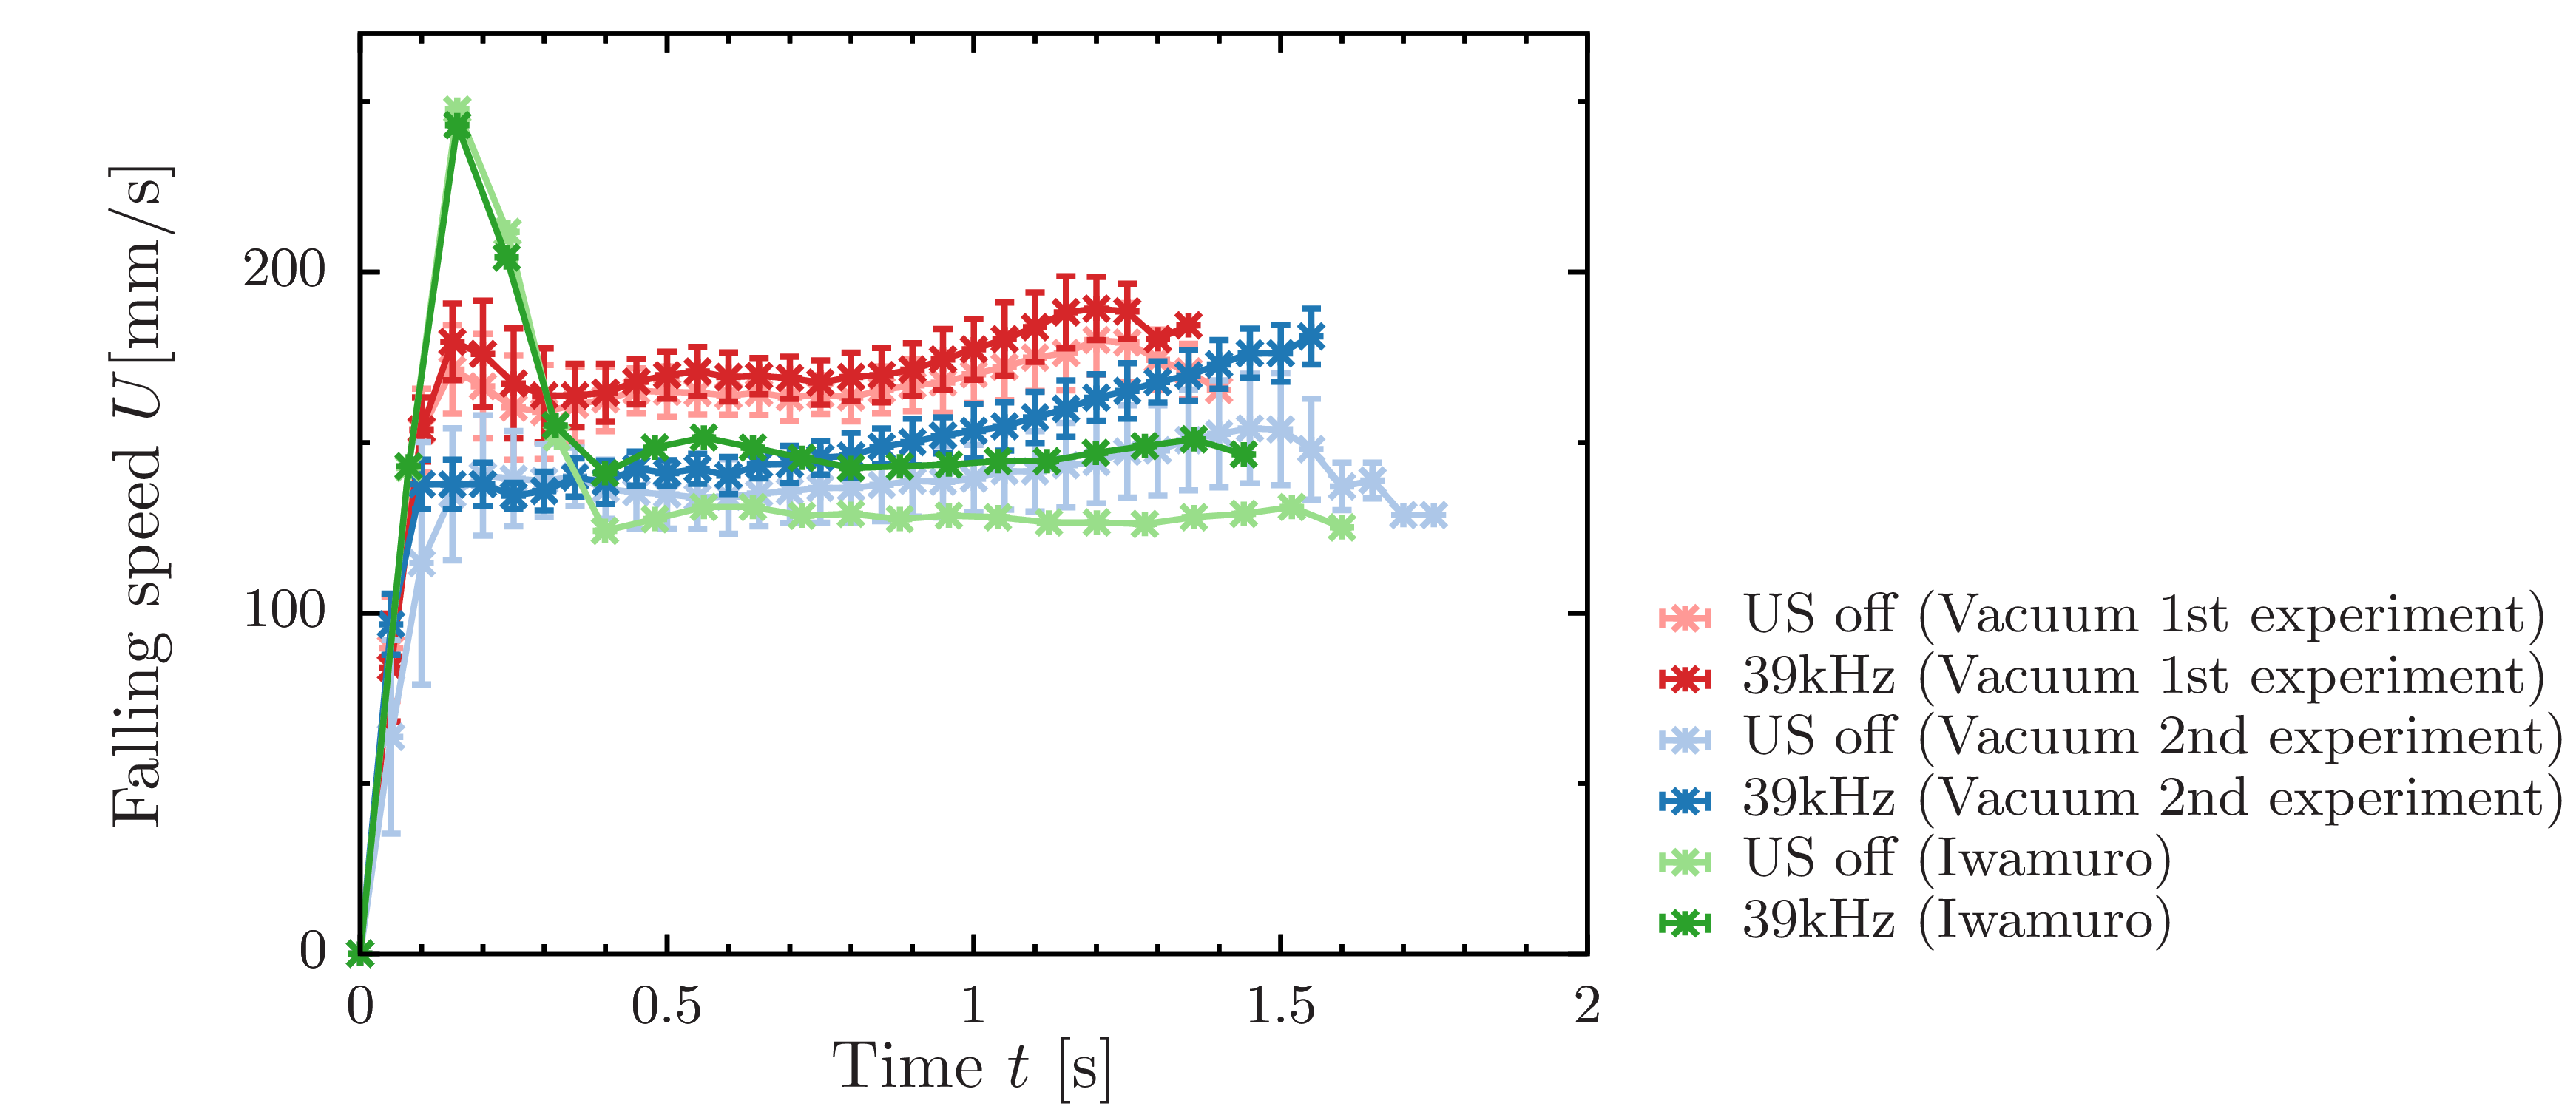
\includegraphics[width=14cm,clip]{X-Appendix/reexp.png}
%     \caption{Falling velocity of a sphere in 1wt.\%PAA solution with and without ultrasound irradiation in tank A (reproducibility check).}
%     \label{fig:re-exp-vaccume}
% \end{figure}
